\documentclass[11pt]{beamer}
\usetheme{Warsaw}
\usepackage[utf8]{inputenc}
\usepackage[english]{babel}
\usepackage{amsmath}
\usepackage{amsfonts}
\usepackage{amssymb}
\usepackage{graphicx}
\usepackage{caption}
\usepackage{booktabs}


%
\author{Nhut-Nam Le}
\title{INTRODUCTION TO MACHINE LEARNING \newline Talk about the paper"Speaker Recognition from Raw Waveform with SincNet"}
\institute{Department of Computer Science, University of Science, VNU} 


%
\setbeamertemplate{caption}[numbered]
% \setbeamertemplate{footline}[frame number]
% footer
\makeatletter
\setbeamertemplate{footline}
{
	\leavevmode%
	\hbox{%
		\begin{beamercolorbox}[wd=1\paperwidth,ht=2.25ex,dp=1ex,right]{institute in head/foot}%
			\usebeamerfont{title in head/foot} 
			\insertframenumber{} / \inserttotalframenumber\hspace*{2ex} 
	\end{beamercolorbox}}%
}
\makeatother
%
\newcommand{\argmax}{\arg\!\max}

\begin{document}
\begin{frame}
	\titlepage
\end{frame}

\begin{frame}{Table of Contents}
	\tableofcontents
\end{frame}

\section{Motivation}
\begin{frame}{Motivation of Speaker Recognition}
	\begin{itemize}
		\item In the field of Speech Recognition, this is a field of research with many real applications such as biometric authentication, forensics, security, speech recognition and speech polarization.
		\item Most state-of-the-art solutions are based on the \textbf{i-vector} representation of speech segments, improvement compared with Gaussian Mixture Model-Universal Background Models.
		\item The development of Deep learning (Deep Neural Networks).
	\end{itemize}
\end{frame}
\section{Problem statments}
\begin{frame}{Problem statments of Speaker Recognition}
	With Speaker Identification task:
	\begin{itemize}
		\item Input: User voice/ speech
		\item Output: User identity data
	\end{itemize}
	With Speaker Verification task:
	\begin{itemize}
		\item Input: User voice/ speech
		\item Output: Accept/ Deny
	\end{itemize}
\end{frame}
\section{Introduction to the paper}
\begin{frame}{Introduction to the paper}
	\begin{itemize}
		\item In this paper, the authors propose a new CNN (Convolutional Neural Networks) Architecture, exploring the first convolutional layer to discover more information in speech signal - called SincNet.
		\item SincNet based on the  parameterized sinc function, for implement band-pass filters
		\item In contrast to standard CNNs, which learn all the elements of each filter, here, SincNet only uses direct low-cutoff frequencies and direct high-learning data with the proposed method.
		\item Compact and efficient at customizing the apps we want.
		\item Great combination between Machine Learning and Digital Signal Processing.
	\end{itemize}
\end{frame}

\section{Problems processing voice signals}
\begin{frame}{Problems processing voice signals}
	\begin{itemize}
		\item The input data - Raw Speech/Audio is high-dimensional data.
		\begin{figure}[H]
			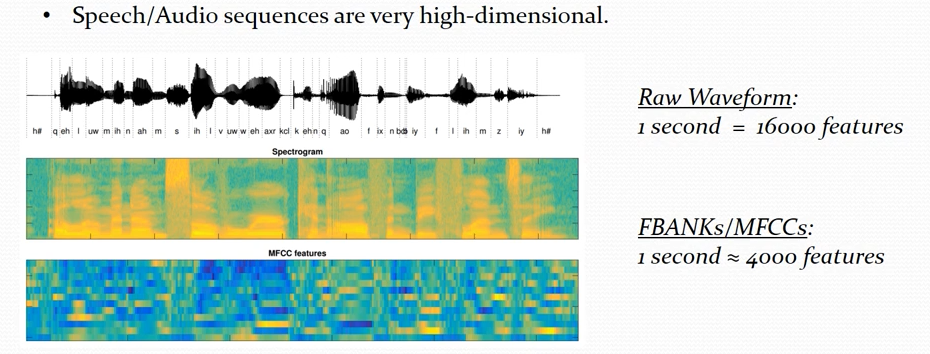
\includegraphics[width=1\linewidth]{images/capture_01.png}
			\caption{A brief introduction to SincNet - Mirco Ravanelli}
			\label{fig:writing-thesis}
		\end{figure}
	\end{itemize}
\end{frame}
\begin{frame}{Problems processing voice signals}
	\begin{itemize}
		\item A problem when we use some smooth techniques with speech sequences.
		\begin{figure}[H]
			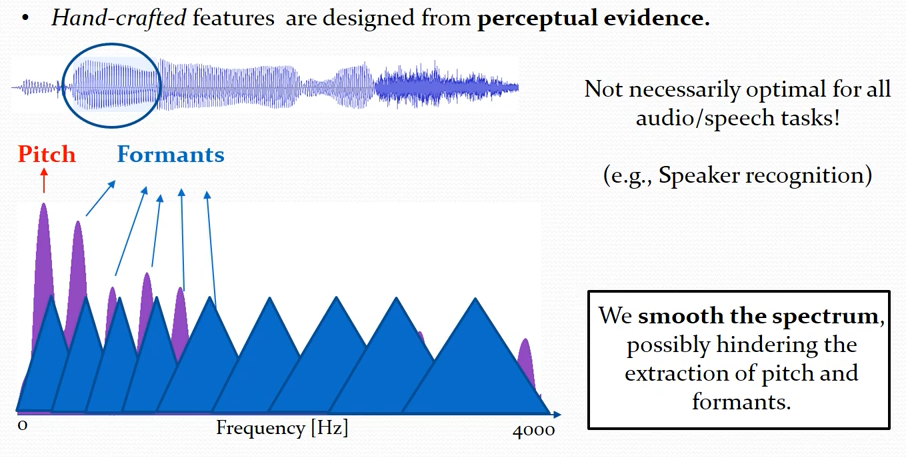
\includegraphics[width=1\linewidth]{images/perceptual_evidence.png}
			\caption{A brief introduction to SincNet - Mirco Ravanelli}
			\label{fig:writing-thesis}
		\end{figure}
	\end{itemize}
\end{frame}
\begin{frame}{Problems processing voice signals}
	\begin{itemize}
		\item CNN filters certainly make some sense for the neural net-
		work, but do not appeal to human intuition, nor appear to lead
		to an efficient representation of the speech signal.
		\begin{figure}[H]
			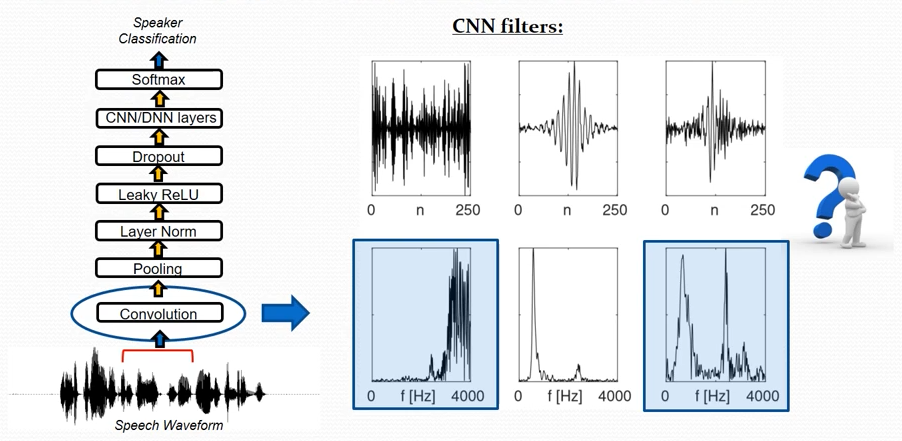
\includegraphics[width=0.95\linewidth]{images/interpretability_problems.png}
			\caption{A brief introduction to SincNet - Mirco Ravanelli}
			\label{fig:writing-thesis}
		\end{figure}
	\end{itemize}
\end{frame}
\begin{frame}{Problems processing voice signals}
	\begin{itemize}
		\item CNN - Vanishing Gradient Problem
		\begin{figure}[H]
			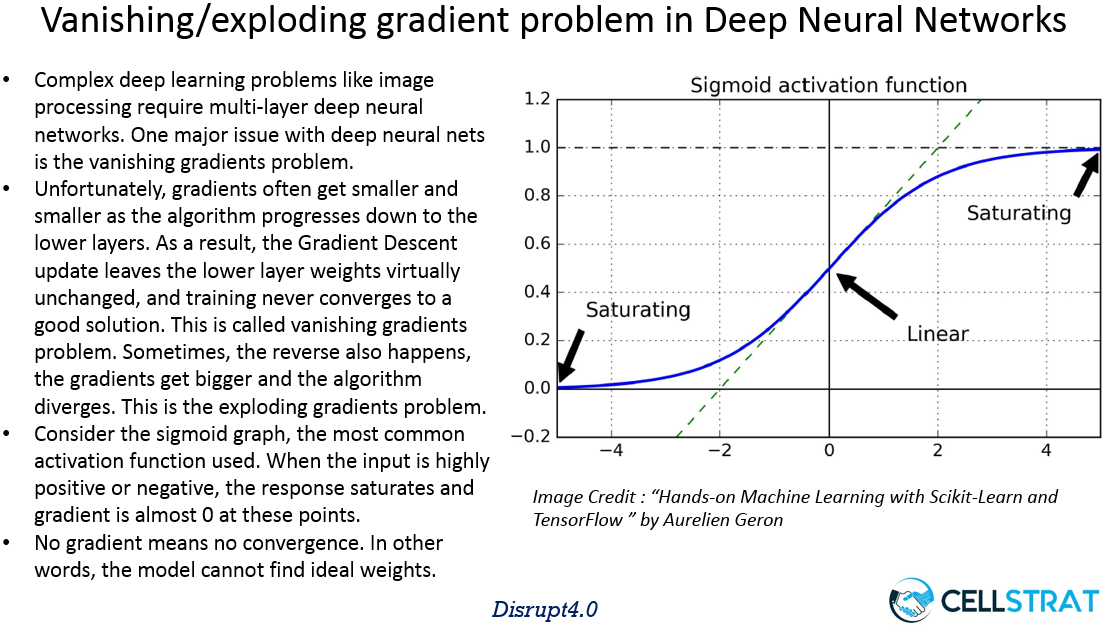
\includegraphics[width=0.95\linewidth]{images/Vanishing-Gradients-in-DNN.png}
			\caption{A brief introduction to SincNet - Mirco Ravanelli}
			\label{fig:writing-thesis}
		\end{figure}
	\end{itemize}
\end{frame}

\section{SincNet Architecture}
\begin{frame}{SincNet}
	\begin{block}{~\vspace{0.7cm}}
		\begin{center}
			\vspace{-0.8cm}
			\begin{tabular}{p{0.45\textwidth}|p{0.45\textwidth}}
				\textcolor{white}{\bf Standard CNN} & \textcolor{white}{\bf SincNet} \\\\
				$y[n] = x[n] * h[n]$ & $y[n] = x[n] * g[n, \theta]$\\
				Learn from all the elements of each filter & Learn from $\theta$ of a predefined kernel\\
			\end{tabular}
		\end{center}
	\end{block}
	\textbf{Problem: How we choose $g(.)$ function?}
\end{frame}
\begin{frame}{SincNet Architecture}
	The idea to build the function $g (.)$ Comes from Digital Signal Processing, based on a bandwidth filter (\textbf{band-pass filters}), with only low-high cutoffs frequencies) are learned.
	\begin{figure}[H]
		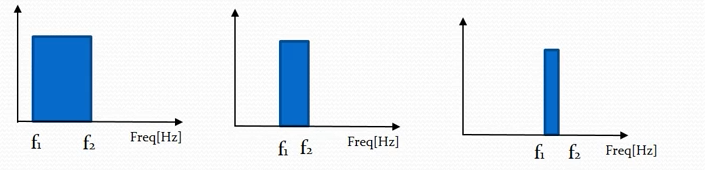
\includegraphics[width=0.9\linewidth]{images/band_passfilters.png}
		\caption{A brief introduction to SincNet - Mirco Ravanelli}
		\label{fig:writing-thesis}
	\end{figure}
\end{frame}
\begin{frame}{SincNet Architecture}
	With $ f_1 $ $ f_2 $ being learned low and high frequency respectively, $ rect (.) $ Is a rectangular function in frequency domain.
	
	$$G[f, f_1, f_2] = rect\left(\frac{f}{2f_2}\right) -  rect\left(\frac{f}{2f_1}\right)$$
	
	To be able to return to the time domain we use the Inverse Fourier transformation:
	
	$$g[n, f_1, f_2] = 2f_2sinc(2\pi f_2 n) - 2f_1sinc(2\pi f_1 n)$$ 
\end{frame}
\begin{frame}{SincNet Filters vs. Standard CNNs}
	\begin{block}{~\vspace{0.7cm}}
		\begin{center}
			\vspace{-0.8cm}
			\begin{tabular}{p{0.45\textwidth}|p{0.45\textwidth}}
				\textcolor{white}{\bf CNN Filters} & \textcolor{white}{\bf SincNet Filters} \\\\
				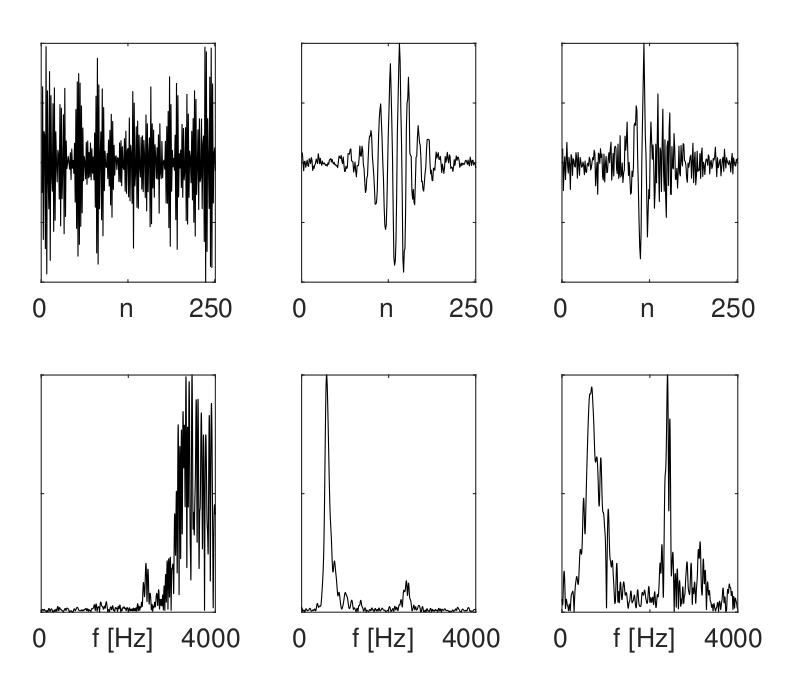
\includegraphics[width=1\linewidth]{images/cnn_filters.png} & 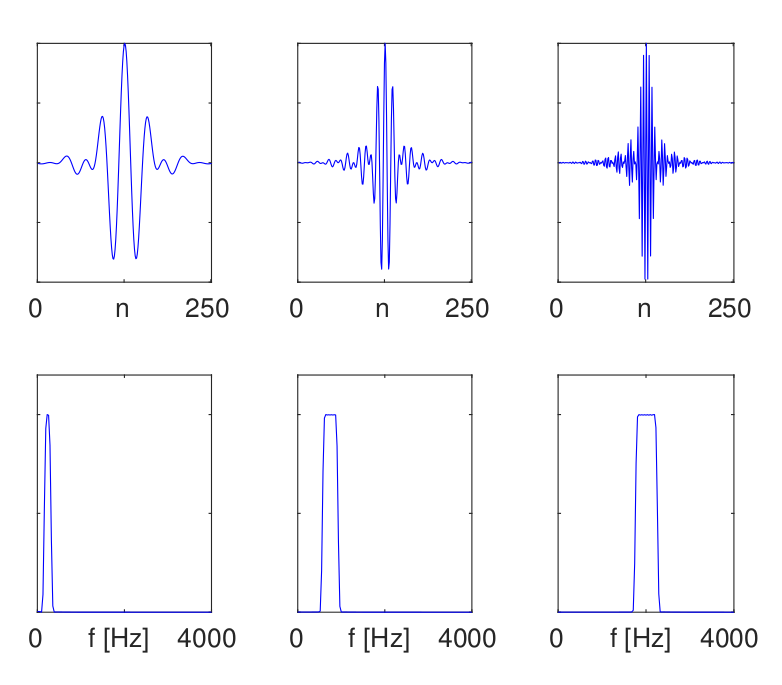
\includegraphics[width=1\linewidth]{images/sincnet_filters.png}\\
			\end{tabular}
		\end{center}
	\end{block}
\end{frame}
\begin{frame}{SincNet Architecture Digram}
	\begin{figure}[H]
		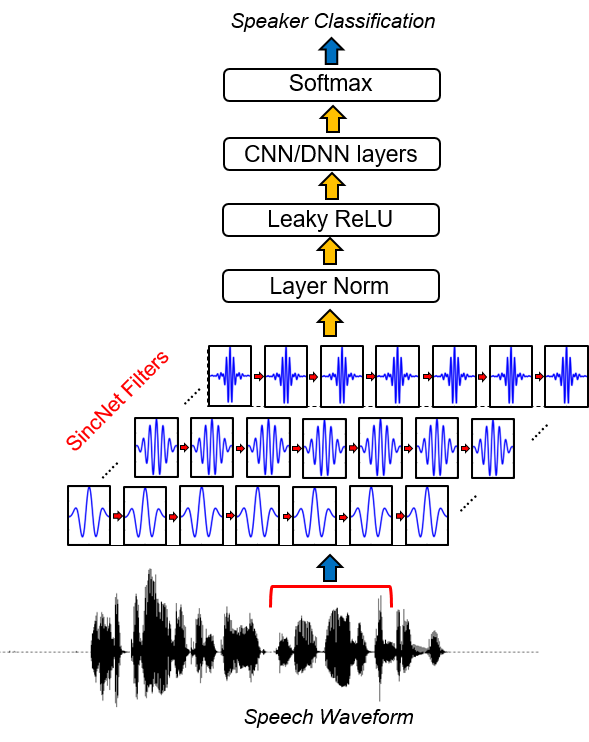
\includegraphics[width=0.4\linewidth]{images/SincNet.png}
		\caption{The SincNet Architecture}
		\label{fig:writing-thesis}
	\end{figure}
\end{frame}
\begin{frame}{SincNet Architecture Properties}
	\begin{columns}
		\begin{column}{0.47\textwidth}
			\begin{figure}[H]
				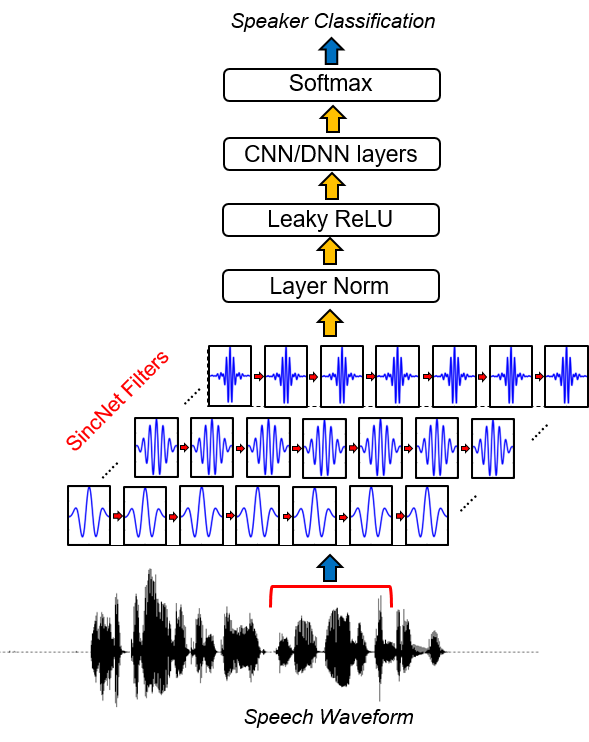
\includegraphics[width=0.9\linewidth]{images/SincNet.png}
			\end{figure}
		\end{column}
		\begin{column}{0.5\textwidth}
			\begin{itemize}
				\item Fast convergence
				\begin{figure}[H]
					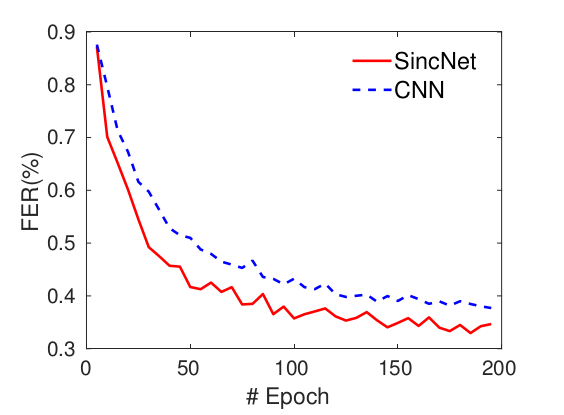
\includegraphics[width=0.9\linewidth]{images/fast_convergence.png}
				\end{figure}
			\end{itemize}
		\end{column}
	\end{columns}
\end{frame}
\begin{frame}{SincNet Architecture Properties}
	\begin{columns}
		\begin{column}{0.47\textwidth}
			\begin{figure}[H]
				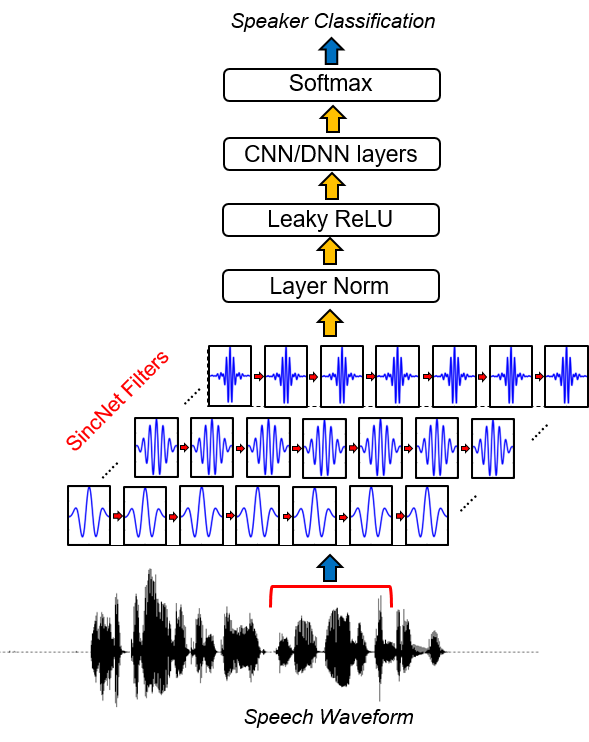
\includegraphics[width=0.9\linewidth]{images/SincNet.png}
			\end{figure}
		\end{column}
		\begin{column}{0.5\textwidth}
			\begin{itemize}
				\item Efficiency
				\begin{figure}[H]
					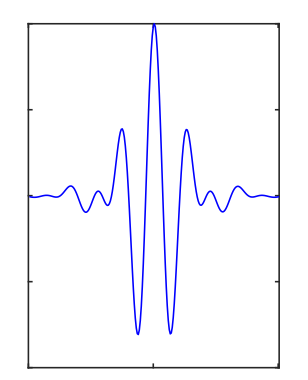
\includegraphics[width=0.45\linewidth]{images/g_symmetric.png}
				\end{figure}
				\item 	The kernel functions $g(.)$ are symmetric, so we only need to do the convolution on a partial filter.
				\item This will save 50 \% of the computation.
			\end{itemize}
		\end{column}
	\end{columns}
\end{frame}
\begin{frame}{SincNet Architecture Properties}
	\begin{columns}
		\begin{column}{0.47\textwidth}
			\begin{figure}[H]
				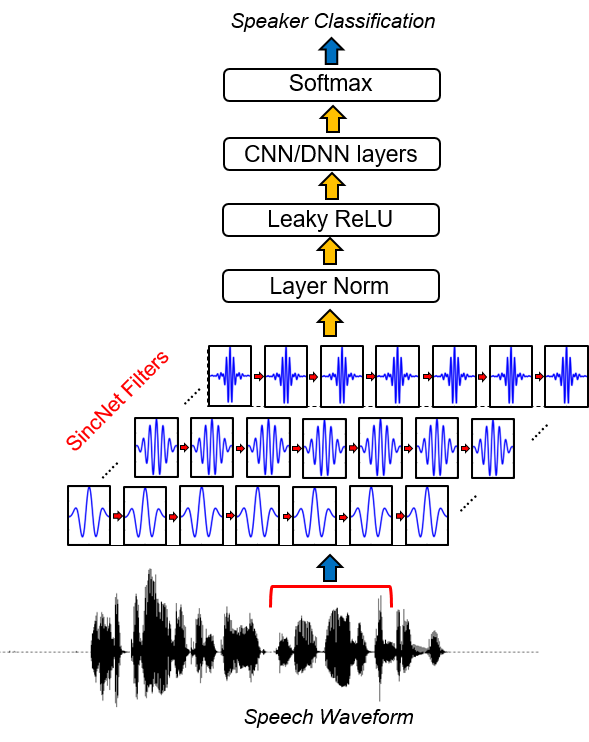
\includegraphics[width=0.9\linewidth]{images/SincNet.png}
			\end{figure}
		\end{column}
		\begin{column}{0.5\textwidth}
			Few Parameters \newline
			Suppose that $F$ is the number of filters, $L$ is the length of each filters.
			\begin{itemize}
				\item With CNN, number of $parameters = F * L$
				\item With SincNet, number of $parameters = 2F$
			\end{itemize}
		\end{column}
	\end{columns}
\end{frame}
\begin{frame}{SincNet Architecture Properties}
	\begin{columns}
		\begin{column}{0.47\textwidth}
			\begin{figure}[H]
				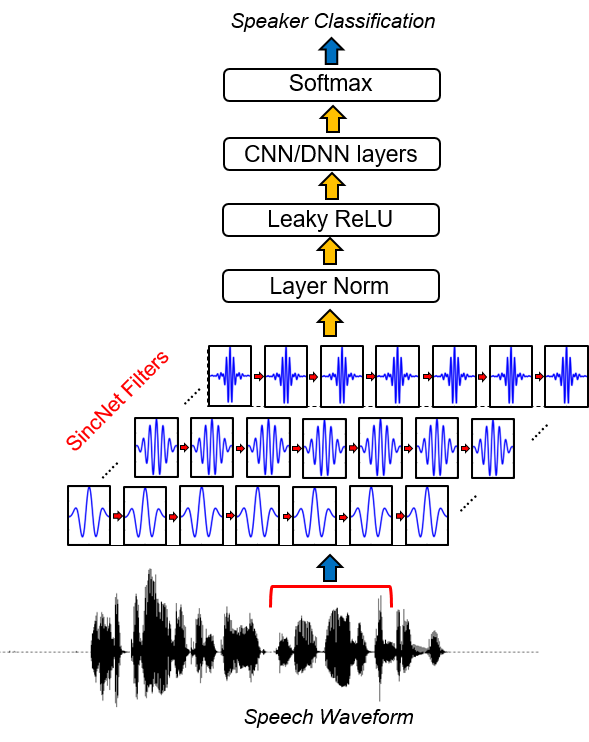
\includegraphics[width=0.9\linewidth]{images/SincNet.png}
			\end{figure}
		\end{column}
		\begin{column}{0.5\textwidth}
			\begin{itemize}
				\item Interpretability
				\begin{figure}[H]
					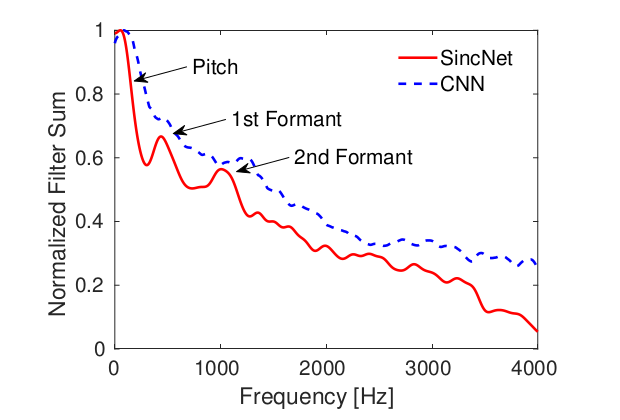
\includegraphics[width=0.9\linewidth]{images/interpretability.png}
				\end{figure}
			\end{itemize}
		\end{column}
	\end{columns}
\end{frame}

\section{Results}
\begin{frame}{Speaker Identification Task}
	\begin{figure}[H]
		\centering
		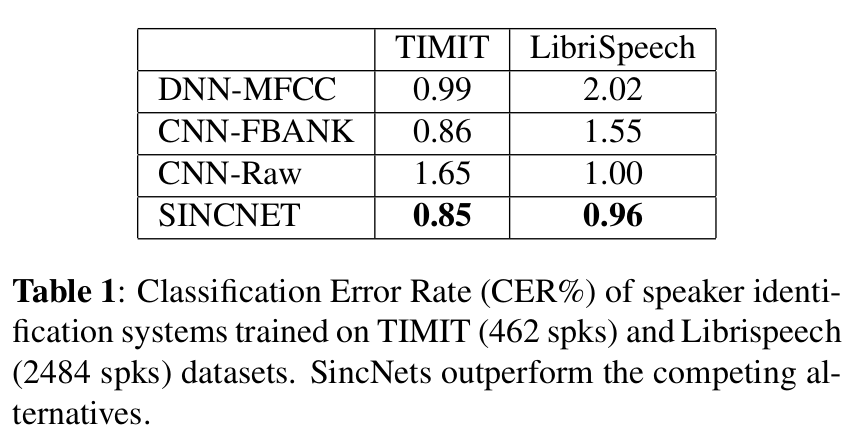
\includegraphics[width=0.75\textwidth]{images/performance_speaker_identification.png}
		\caption{esult table of Speaker Identification Task on TIMIT and LibriSpeech}
		\label{fig:writing-thesis}
	\end{figure}	
\end{frame}
\begin{frame}{Speaker Verification Task}
	\begin{figure}[H]
		\centering
		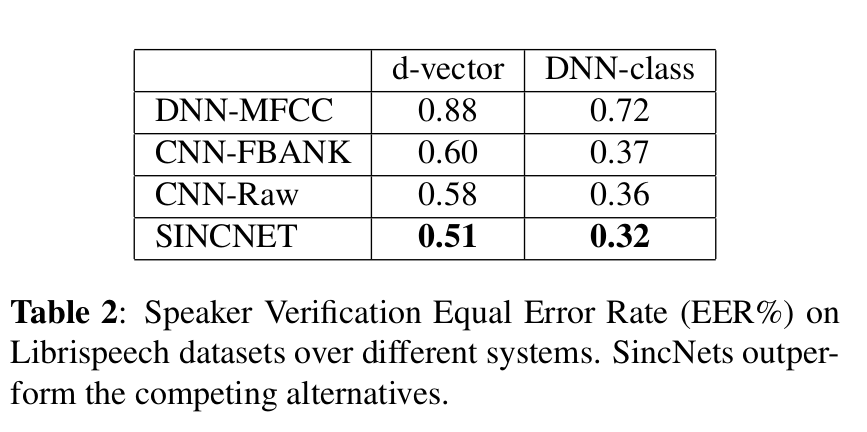
\includegraphics[width=0.75\textwidth]{images/performance_speaker_verification.png}
		\caption{Result table of Speaker Verification Task on TIMIT and LibriSpeech}
		\label{fig:writing-thesis}
	\end{figure}	
\end{frame}
\begin{frame}{Speaker Verification with i-vectors evaluate}
	The best \textbf {i-vector} system of the authors achieved \textbf{EER = 1,1 \%}, \textbf{quite far from what was achieved with the DNN} system.
\end{frame}
\begin{frame}{Speaker Recognition on DIRHA}
	\begin{figure}[H]
		\centering
		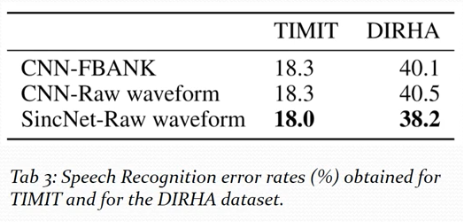
\includegraphics[width=0.65\textwidth]{images/sr_sincnet_result.png}
		\caption{Result table of Speaker Recognition with SincNet on DIRHA}
		\label{fig:writing-thesis}
	\end{figure}	
\end{frame}
\section{References}
\begin{frame}{References}
	\nocite{*}
	\bibliography{references.bib}\newpage\cleardoublepage
	\bibliographystyle{plain}
\end{frame}
\begin{frame}{Q\&A}
	\begin{center}
		\Huge Thank you
	\end{center}
\end{frame}

\end{document}